%!TEX root = ../crowd_hierarchies_v.1.3.tex


\section{Experimental Evaluation}
\label{sec:exps}
In this section we present an empirical evaluation of our proposed algorithmic framework. The main questions we seek to address are: (1) how the proposed querying policy algorithm compares against baselines for maximizing the number of extracted entities under a specific budget, (2) how the different gain estimators presented in \Cref{sec:gainestimators} compare with each other, and (3) how the proposed querying policy algorithm exploits the structure of the input domain to construct the set of available actions.

We empirically study these questions using both real and synthetic datasets. First, we discuss the experimental methodology, and then we describe the data and results that demonstrate the effectiveness of our framework on crowdsourced entity extraction. The evaluation is performed on an Inter(R) Cored(TM) i7 3.7 GHz 32GB machine; all algorithms are implemented in Python 2.7. 

\vspace{5pt}\noindent\textbf{Gain Estimators:} We evaluate the following gain estimators:
\squishlist
\item Chao92Shen: This estimator combines the methodology proposed by Chao~\cite{chao:1992} for estimating the number of unseen species  with Shen's formula, i.e., \Cref{eq:shen}. This estimator was also used by Trushkowsky et al.~\cite{trushkowsky:2013}.
\item HwangShen: This estimator combines the regression based approach proposed by Hwang and Shen~\cite{hwang:2010} for estimating the number of unseen species with Shen's formula. 
\item NewRegr: This estimator corresponds to the new regression based technique proposed in \Cref{sec:newestim}.
\squishend
All estimators were coupled with bootstrapping to estimate their variance. Computing the variance of each estimator is required to retrieve an upper bound on the return of a query as shown in \Cref{eq:upper}.

\vspace{5pt}\noindent\textbf{Entity Extraction Algorithms:} We evaluate the following algorithms for crowdsourced entity extraction:
\squishlist
\item Rand: This algorithm executes random queries until all the available budget is used. It selects a random node from the input poset $\hierarchy$ and a random query configuration $q(k,l)$ from a list of pre-specified $k$, $l$ value combinations. We expect Rand to be effective for extracting entities in small and dense data domains that do not have many sparsely populated nodes.
\item RandL: This algorithm executes random queries {\em only at the lowest level nodes} (i.e., leaf nodes) of the input poset $\hierarchy$ until all the available budget is used. It selects a random leaf node and a random query configuration $q(k,l)$ from a list of pre-specified $k$, $l$ value combinations. We expect RandL to be effective for {\em shallow} data domains when the majority of nodes corresponds to leaf nodes. And similar to Rand, the performance of RandL is expected to be reasonable for small and dense data domains without sparsely populated nodes.
\item BFS: This algorithm performs a breadth-first traversal of the input poset $\hierarchy$, executing one query at each node. The query configuration is randomly selected from a list of pre-specified $k$, $l$ value combinations. This algorithm promotes exploration of the action space when extracting entities. It also takes into account the structure of the input domain but is agnostic to sparsely populated nodes of the input $\hierarchy$.
\item GSChao, GSHWang, GSNewR: These algorithms correspond to our proposed querying policy algorithm shown in \Cref{sec:heuristic} coupled with Chao92Shen, HwangShen and NewRegr respectively.
\item GSExact: This algorithm is used as a near-optimal, omniscient baseline that allows us to see how far off our algorithms are from an algorithm with perfect information. In particular, we combine the algorithm proposed in \Cref{sec:heuristic} with an exact computation of the return or gains from queries. More precisely, the algorithm proceeds as follows: At each round we speculatively execute each of the available actions (i.e., all query configurations across all nodes) and select the one that results in the largest number of return to cost ratio. Since the return of each query is known, the algorithm is not coupled with any of the aforementioned estimators.
\squishend

Rand, RandL and BFS promote the exploration of the action space when extracting entities, while the other algorithms balance exploration with exploitation. For the results reported below, we run each algorithm ten times and report the average gain achieved under the given budget.

\vspace{5pt}\noindent\textbf{Querying Interface:} For all datasets we consider generalized queries $q(k,l)$ of the type ``Give me $k$ more entities that satisfy certain conditions and are not present in an exclude list of size $l$". The conditions correspond to matching the attribute values associated with a node from the input poset. The  configurations considered for $(k,l)$ are $\{(5,0), (10,0), (20,0), (5,2), (10,5), (20,5), (20,10)\}$. Larger values of $k$ or $l$ were deemed unreasonable for crowdsourced queries. The gain of a query is computed as the number of new entities extracted. The cost of each query is computed using an additive model comprised by three partial cost terms that depend on the characteristics of the query. 

The three partial cost terms are: (i) {\sf CostK} that depends on the number of responses $k$ requested from a user, (ii) {\sf CostL} that depends on the size of the exclude list $l$ used in the query, and (iii) {\sf CostSpec} that depends on the {\em specificity} of the query $q_s$, e.g., we assume that queries that require users to provide more specialized entities such as a ``Give me one concert for New York on the 17th of Nov" cost more than more generic queries such as ``Give me one concert in New York". More formally, we define the specificity of a query to be equal to the number on attributes assigned non-wildcard values for the node $u \in \hierarchy$ the query corresponds to. 

For each of the cost terms we assume a maximum cost of \$1 realized by considering the maximum value of the corresponding input variable. The overall cost for a query $q(k,l)$ with specificity $s$ is computed as:

{\small
\begin{equation}
Cost(q) = \alpha \cdot \frac{k}{\mbox{max. query size}} + \beta \cdot  \frac{l}{\mbox{max. ex. list size}} + \gamma \cdot  \frac{s}{\mbox{max. specificity}} \nonumber
\end{equation}}

The cost of a query should be significantly increased when an exclude list is used, thus we require that $\beta$ is set to a larger value than $\alpha$ and $\gamma$. For the results reported below, we set $\alpha = \gamma = 1$ and $\beta = 5$. Similar results were observed for other settings but are omitted due to space limitations.

\subsection{Synthetic Data Experiments}
\label{sec:synthetic}
First, we evaluate the proposed framework on extracting entities from a large domain. We consider the event dataset collected from Eventbrite. As described in \Cref{sec:intro}, the poset corresponding to the Eventbrite domain contains 8,508,160 nodes with 57,805 distinct events overall. However, only 175,068 nodes are populated leading to an rather sparsely populated domain. Due to lack of popularity proxies for the extracted events, we assigned a random {\em popularity value} in $(0,10]$ to each event. These weights are used during sampling to form the actual popularity distribution characterizing the population of each node in the poset. 

\noindent\textbf{Results:}  We evaluate the performance, in terms of number of entities extracted, for the different extraction algorithms described above, across a range of different budgets. We run each algorithm ten times and report the average number of unique events extracted as well as the corresponding standard error. The results are shown in \Cref{fig:ebextraction}. As can be seen, all of our proposed algorithms, i.e., GSChao, GSHwang, GSNewR outperform the baselines under consideration exhibiting an improvement of at least 2X on the total number of unique events extracted. For example, for budget = \$50, our schemes all extracted greater than 500 events while Rand and RandL extracted 1.1 and 0.2 events and BFS extracted 207.7 events, an improvement of over 140\%. Moreover, for smaller budgets we observe that these algorithms perform comparably to GSExact that has ``perfect information'' to the gain of each query, typically giving half the number of entities that GSExact extracts. Note that our estimators have access to few samples and sparse information; the fact that we are able to get this close to GSExact is notable.

\begin{figure}[h]
	\begin{center}
	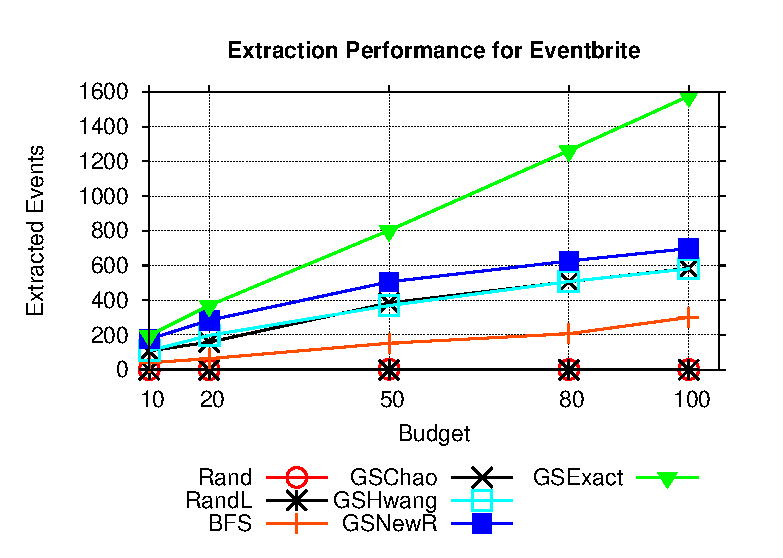
\includegraphics[clip,scale=0.5]{figs/ebExtractionAll.eps}
	\caption{The number of events extracted by different algorithms for the Eventbrite data domain and different budgets.}
	\label{fig:ebextraction}
	\end{center}
	\vspace{-20pt}
\end{figure}

%\begin{figure*}[ht]
%\begin{center}
%        \subfigure{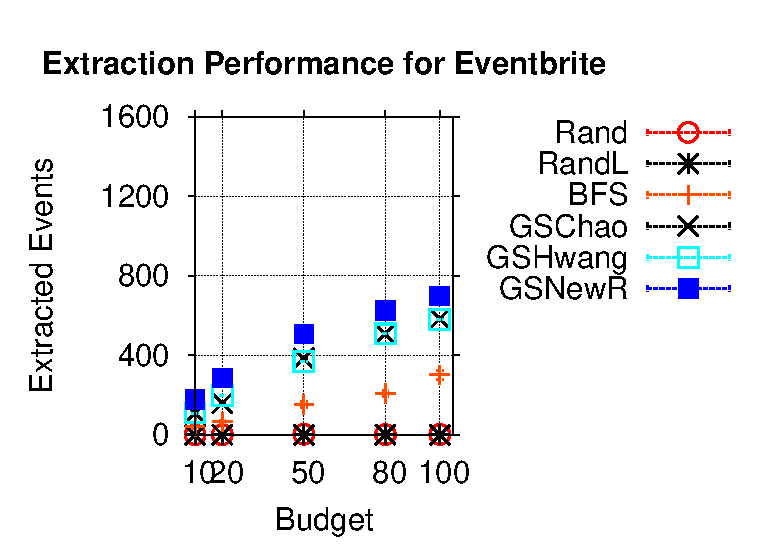
\includegraphics[clip,scale=0.5]{figs/ebExtraction.eps} \label{fig:ebextractiona}}
%        \subfigure{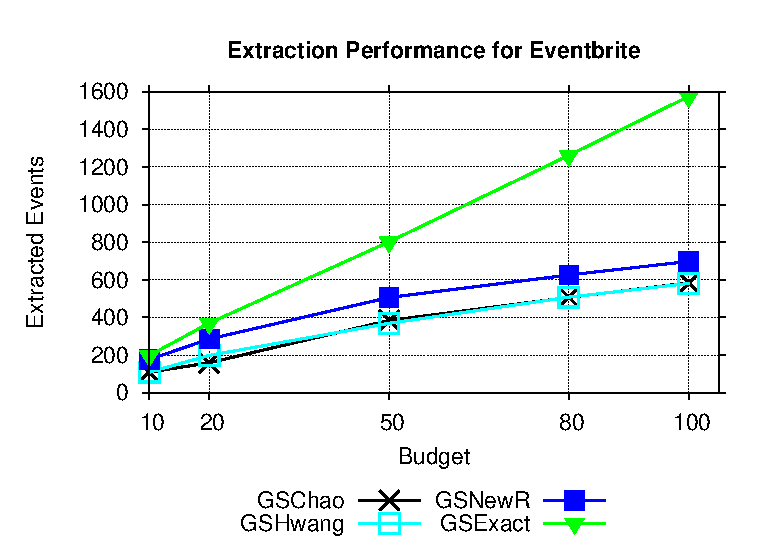
\includegraphics[clip,scale=0.5]{figs/ebExtractionGS.eps} \label{fig:ebextractiona}}
%\end{center}
%\vspace{-10pt}
%\caption{The number of events extracted by different algorithms for the Eventbrite data domain and different budgets.}
%\label{fig:ebextraction}
%\vspace{-10pt}
%\end{figure*}

The poor performance of Rand and RandL is due to the sparsity of the Eventbrite data domain. Regarding BFS, we see that it exhibits better performance than Rand and RandL by exploiting the structure of the underlying domain. However, since BFS is agnostic to the cost of the issued queries as well as to sparsely populated areas of the underlying poset, it can only extract a limited number of events. On the other hand, our proposed techniques were able to extract significantly more tuples as they both exploit the structure of the poset and optimize for the cost of the issued queries. Finally, we point out that GSNewR that combines the proposed poset traversal algorithm with our new regression-based gain estimator was able to outperform GSChao and GSHwang. 

To further understand the relative performance of GSChao, GSHwang and GSNewR, we evaluate the performance of the gain estimators described above at predicting the number of new retrieved events for different query configurations. We choose ten random nodes from Eventbrite each containing more than 5,000 events. For each of the nodes and each of the available query parameter configurations $(k,l)$, we execute ten queries of the form ``Give me $k$ items from node $u \in \hierarchy$ that are not included in an exclude list of size $l$". As mentioned in \Cref{sec:excludelist} the exclude list for each query is constructed following a randomized approach. 

We measure the performance of each estimator by considering the absolute relative error between the predicted return and the actual return of the query. In \Cref{tab:eventesterror}, we report the relative error for each of the three estimators averaged over all points under consideration. As shown, all three estimators perform equivalently with the new regression based technique slightly outperforming Chao92Shen and HwangShen for certain types of queries. For example, for $k = 10, l = 5$, Chao92Shen has a relative error of 0.58, HwangShen had a relative error of 0.7, and NewRegr had a relative error of 0.56. We attribute the improved extraction performance of GSNewR to these improved estimates. The relatively large values for relative errors are justified as the retrieved samples correspond to a very small portion of the underlying population for each of the points. This is a well-known behavior for non-parametric estimators and studied extensively in the species estimation literature~\cite{hwang:2010}. 

\begin{table}
\scriptsize\center
\caption{Average absolute relative error for estimating the gain of different queries for Eventbrite.}
\label{tab:eventesterror}
\begin{tabular}{|c|c|c|c|c|}
\hline
\textbf{Q. Size $k$} & \textbf{EL. Size $l$} & \textbf{Chao92Shen} & \textbf{HwangShen} & \textbf{NewRegr} \\ \hline
5 & 0 & 0.470 & 0.500 & 0.427 \\
5 & 2 & 0.554 & 0.612 & 0.567\\
10 & 0 & 0.569 & 0.592 & 0.544\\
10 & 5 & 0.580 & 0.696 & 0.559\\
20 & 0 & 0.642 & 0.756 &0.601\\
20 & 5 & 0.510 & 0.60 & 0.519 \\
20 & 10 & 0.653 & 0.756 & 0.631\\
\hline
\end{tabular}
\vspace{-10pt}
\end{table}

\subsection{Real Data Experiments}
\label{sec:realdata}
Since the performance of the baseline algorithms is significantly affected by the sparsity of the Eventbrite data domain, we choose to further evaluate the performance of the extraction algorithms for a more dense domain, that we constructed ourselves. We used Amazon's Mechanical Turk~\cite{mturk} to collect a real-world dataset, targeted at extracting ``people in the news''. 

We asked workers to extract the names of people belonging to four different types from five different news portals. The people types we considered are ``Politicians", ``Athletes", ``Actors/Singers" and ``Industry People". The news portals we considered are ``New York Times", ``Huffington Post", ``Washington Post", ``USA  Today" and ``The Wall Street Journal". This data domain, referred to as the People's domain, is essentially characterized by the type of the individual and the news portal. Workers were paid \$0.20 per HIT. We issued 20 HITS for each leaf node of the domain's poset, resulting in 600 HITS in total. After manually curating name misspelling's, we extracted 1,245 unique people in total. \Cref{tab:ptypedata} shows the number of distinct entities for the different values of the people-type and news portal attributes. Finally, the popularity value of each extracted entity was assigned to be equal to the number of times it appeared in the extraction result. The values are normalized during sampling time to form a proper popularity distribution. Collecting a large amount of data in advance from Mechanical Turk and then simulating the responses of human workers by revealing portions of this dataset allows us to compare different algorithms on an equal footing; this approach is often adopted in the evaluation of crowdsourcing algorithms~\cite{DBLP:journals/pvldb/ParameswaranBG0PW14, marcus:2011,trushkowsky:2013}.

\begin{table}
\scriptsize\center
\caption{The population characteristics for the People's data.}
\label{tab:ptypedata}
\begin{tabular}{|c|c|}
\hline
\textbf{Person Type} & \textbf{People} \\ \hline
Industry People & 743 \\
Athletes & 743 \\
Politicians & 748 \\
Actors/Singers & 744 \\ \hline
\end{tabular}
\quad
\begin{tabular}{|c|c|}
\hline
\textbf{News Portal} & \textbf{People} \\ \hline
WSJ & 594 \\
WashPost & 597 \\
NY Times & 595 \\
HuffPost & 599 \\
USA Today & 593 \\ \hline
\end{tabular}
\vspace{-10pt}
\end{table}


\vspace{5pt}\noindent\textbf{Results}: We first evaluate the performance of the different extraction algorithms. Similarly to Eventbrite we run each algorithm ten times and report the average performance. The results are shown in \Cref{fig:poextraction}. As shown our proposed techniques (i.e., GSChao, GSHwang and GSNewR) still outperform Rand, RandL and BFS. However, we see that the performance improvement compared to the baselines is smaller compared to Eventbrite. The reason is that the input domain is dense and all nodes of the input poset are populated, so even random techniques may ``get lucky'' fairly often. Even so, the number of nodes extracted by all our proposed techniques is typically 100\% greater than that of the other techniques for small budgets and 54\% for larger ones.

\begin{figure}[h]
	\vspace{-10pt}
	\begin{center}
	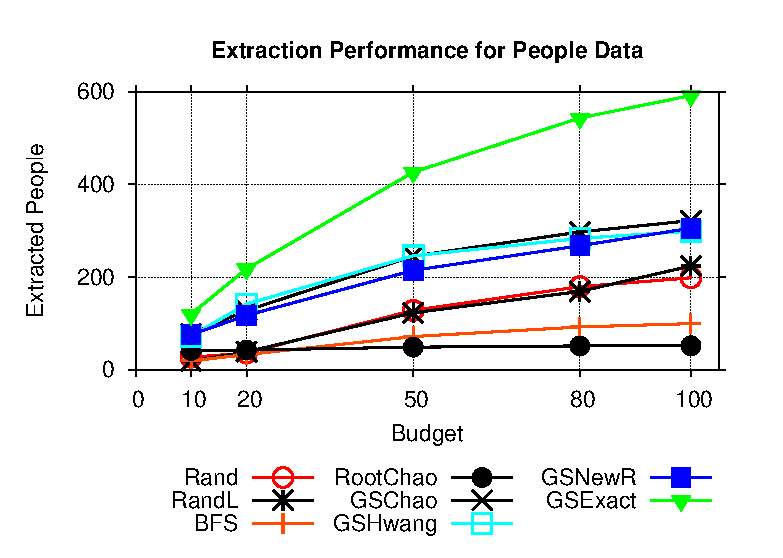
\includegraphics[clip,scale=0.5]{figs/poExtraction.eps}
	\caption{The number of people extracted by different algorithms for the People data domain and different budgets.}
	\label{fig:poextraction}
	\end{center}
	\vspace{-15pt}
\end{figure}

We also observe that issuing random extraction queries at the nodes of the poset outperforms BFS for a significant margin as the available budget increases. This behavior is expected in dense small domains where all the available nodes are populated. Notice that this approach corresponds to a querying policy that focuses purely on exploring different queries. However, exploiting previously obtained information and balancing exploration and exploitation of the possible actions (i.e., following the proposed poset traversal algorithm) leads to superior performance. We further notice that GSChao does better than GSNewR in this case, unlike the previous case. This is because the Chao92Shen estimator performs better when the retrieved samples correspond to a larger portion of the underlying population (i.e., when operating under a large budget), as we see below. 

Next, we evaluate the performance of the gain estimators. As before, we issue ten queries to different nodes of the input poset for all available query configurations. Since the input poset is small, we issued ten queries over all nodes. For each gain estimator and query configuration, we computed the average relative error, comparing the estimated query return with the actual query return. The results are shown in \Cref{tab:peopleesterror}. Again, we observe that for smaller query sizes the regression technique proposed in this paper offers better gain estimates. However, as the query size increases, and hence, a larger portion of the underlying population is observed Chao92Shen outperforms both regression based techniques. Thus, we are able to explain the performance difference between GSChao and the other two algorithms.

\begin{table}[h]
\vspace{-10pt}
\scriptsize \center
\caption{Average absolute percentage error for estimating the gain of different queries for the People's data domain.}
\label{tab:peopleesterror}
\begin{tabular}{|c|c|c|c|c|}
\hline
\textbf{Q. Size $k$} & \textbf{EL. Size $l$} & \textbf{Chao92Shen} & \textbf{HwangShen} & \textbf{NewRegr} \\ \hline
5 & 0 & 0.295 & 0.299 & 0.228\\
5 & 2 & 0.163 &  0.156 & 0.144\\
10 & 0 &  0.306 & 0.305 & 0.277\\
10 & 5 &  0.341 & 0.349 & 0.293\\
20 & 0 &  0.359& 0.371 & 0.467 \\
20 & 5 &  0.402 & 0.418 & 0.493\\
20 & 10 & 0.405 & 0.428 & 0.638\\
\hline
\end{tabular}
\vspace{-5pt}
\end{table}


We next explore how our different algorithms traverse the lattice, and how they use different query configurations, relative to GSExact. We begin by considering how many queries these algorithms issue at various levels of the lattice. In Figure~\ref{fig:level}, we plot the different number of queries issued at various levels by our algorithms when the budget is set to 10 and 100 respectively. \agp{add a couple of lines about how ..} Then, in Figures~\ref{fig:queryconf10} and \ref{fig:queryconf100}, we plot the different query configurations by our algorithms when the budget is set to 10 and 100 respectively. 


\begin{figure}[h]
	\vspace{-10pt}
    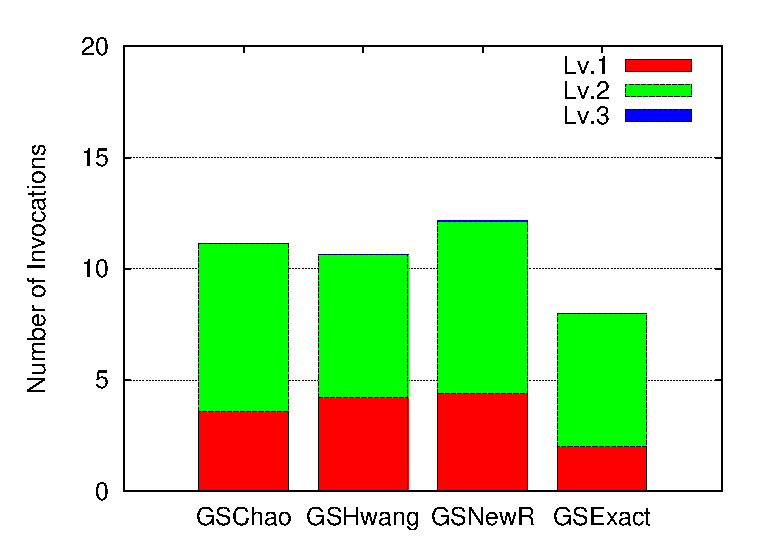
\includegraphics[clip,scale=0.32]{figs/levelBudget10.eps}
	\hspace{-10pt}
	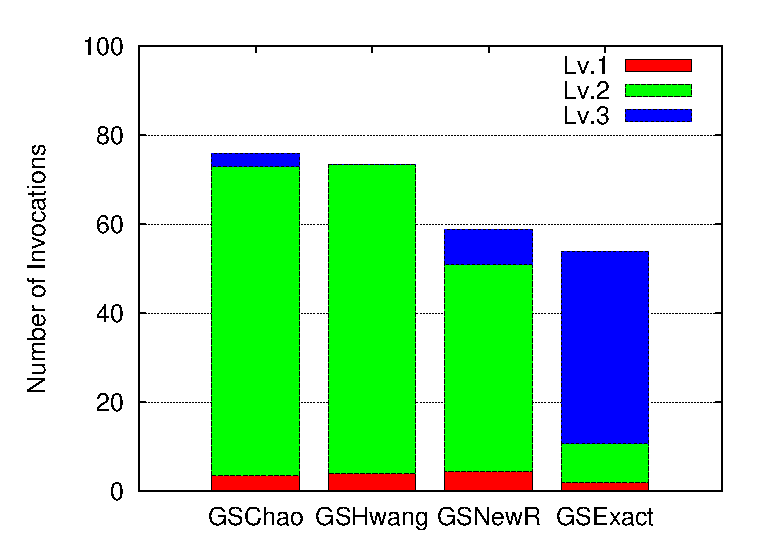
\includegraphics[clip,scale=0.32]{figs/levelBudget100.eps}
	\vspace{-10pt}
	\caption{The different number of queries issued at different levels used when budget is set at 10 or 100.}\label{fig:level}
	\vspace{-10pt}
\end{figure}

\begin{figure}[h]
	\vspace{-5pt}
    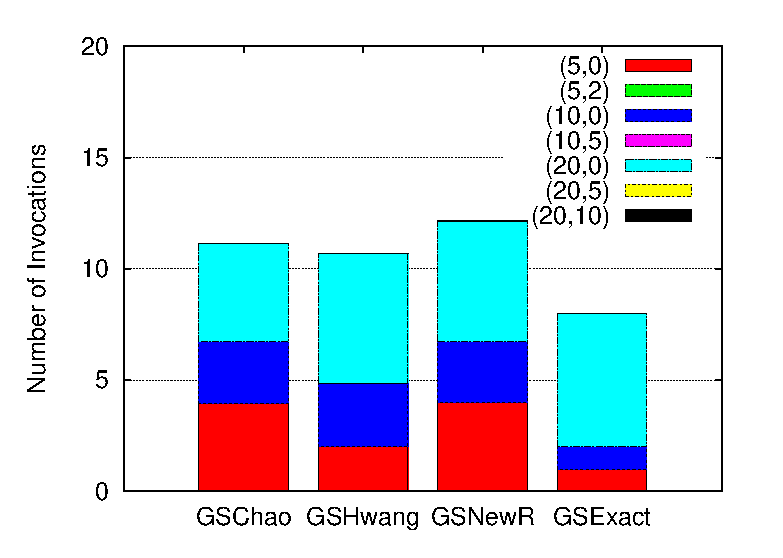
\includegraphics[clip,scale=0.32]{figs/queryConfBudget10.eps}
	\hspace{-10pt}
	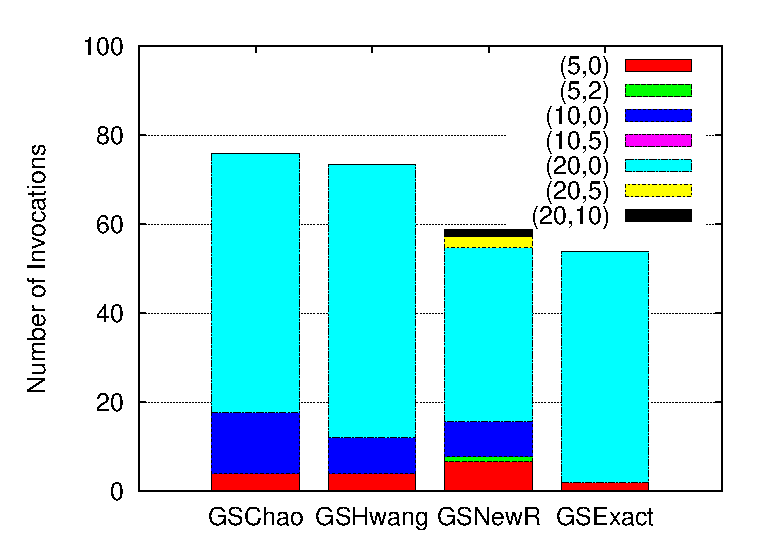
\includegraphics[clip,scale=0.32]{figs/queryConfBudget100.eps}
	\vspace{-10pt}
	\caption{The different query configurations used when budget is set at 10 or 100.}\label{fig:queryconf}
	\vspace{-15pt}
\end{figure}



\subsection{Take-Away Points}
We have the following recommendations based on the experimental results.
\squishlist
\item Exploiting the structure of the entity extraction domain is effective for maximizing the total number of extracted entities. Moreover, balancing the exploration of queries for non-observed nodes of the poset with queries over observed nodes of the poset is crucial.
\item For sparse domains, e.g.., domain specified by large posets with a small number of populated nodes, one should resort to regression based techniques for estimating the expected gain of further queries as they result in better performance. However, for dense domains the Chao92Shen estimator results in better performance as a larger portion of the underlying population can be sampled. The size of the input domain and its sparsity are known in advance to the designer of the querying interface. 
\item For small budgets the proposed estimator-based poset traversal algorithms (i.e., GSChao, GSHwang and GSNewR) exhibit comparable performance with a traversal algorithm that has oracle access to the gain of each query to be issued. For larger budgets we observe that our algorithms are at most 2.2x away from this adaptive querying strategy with perfect information.
\squishend